\section{Conception\label{sec:conception}}

This chapter describes the solution concept and all aspects that were investigated to derive it.
The investigation includes the following activities:

First, the problem statement from Chapter \ref{sec:introduction} is revisited and further refined using information derived from concrete use cases, internal documents and from relevant literature.
Then, the elicited information is analyzed in detail to derive customization operations and criteria for the evaluation and selection of appropriate customization mechanisms that have been introduced in Chapter \ref{sec:foundation}. Finally, the solution concept is formalized.


\subsection{Refined problem statement}
The master's thesis aims to address the challenges of configuring simulations in the automotive industry through the use of semantic technology. The focus is on the development of an expert system that utilizes the metadata of existing simulations to facilitate the creation of new simulations. This solution aims to streamline the configuration process and make it more efficient and accessible, especially for inexperienced simulation engineers.

Here are a few use cases that can be derived from the problem raised by this thesis.

\begin{itemize}
    \item \textbf{New simulation configuration}: When a new simulation needs to be created, the system suggests relevant configurations based on previous simulations with similar goals or constraints, leveraging the semantic relationships embedded in the metadata. This can significantly reduce configuration time and ensure consistency with best practice.
    \item \textbf{Knowledge transfer}: The system serves as a knowledge repository that captures and stores information about previous simulations and their configurations. This allows new engineers to access valuable insights and learn from previous projects, shortening the learning curve and promoting knowledge sharing within the team.
    \item \textbf{Error prevention}: Semantic validation rules ensure that new configurations adhere to the defined guidelines and restrictions. This avoids errors and inconsistencies that could lead to inaccurate simulation results.
    \item \textbf{Configuration optimization}: The system can analyze previous simulation data and suggest optimized configurations based on performance metrics, allowing engineers to achieve better results with less effort.
\end{itemize}


\subsection{Simulation's Architecture}
Figure[] shows a general problem-solving diagram, illustrating how a problem might be handled using CAE methods. Above each phase is the sequence of different steps.\\

\begin{figure}[H]
    \centering
    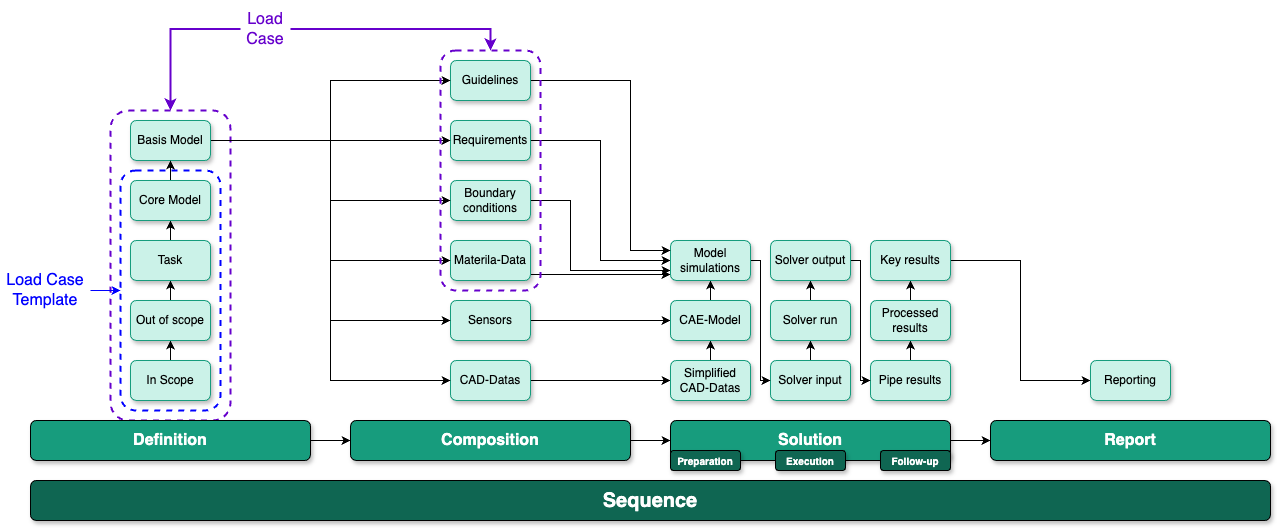
\includegraphics[width=\textwidth]{images/Concept-cae-process.drawio.png}
    \caption{\label{fig:cea-proc}  The CAE core process, illustrated with the stages of a general problem-solving scheme. [ ]}
\end{figure}

Based on the elements and steps involved in this process, a simulation ontology will be created. This will enable us to capture and formalize the elements involved in the configuration process, as well as the interdependencies between them. Particularly important in the context of this thesis are the elements involved in the “Definition” and “Composition” stages, as these lead to a "CAE-Model". Figure[] shows a UML diagram representing the information extracted from Figure[] and the relationships between them.\\

\begin{figure}[H]
    \centering
    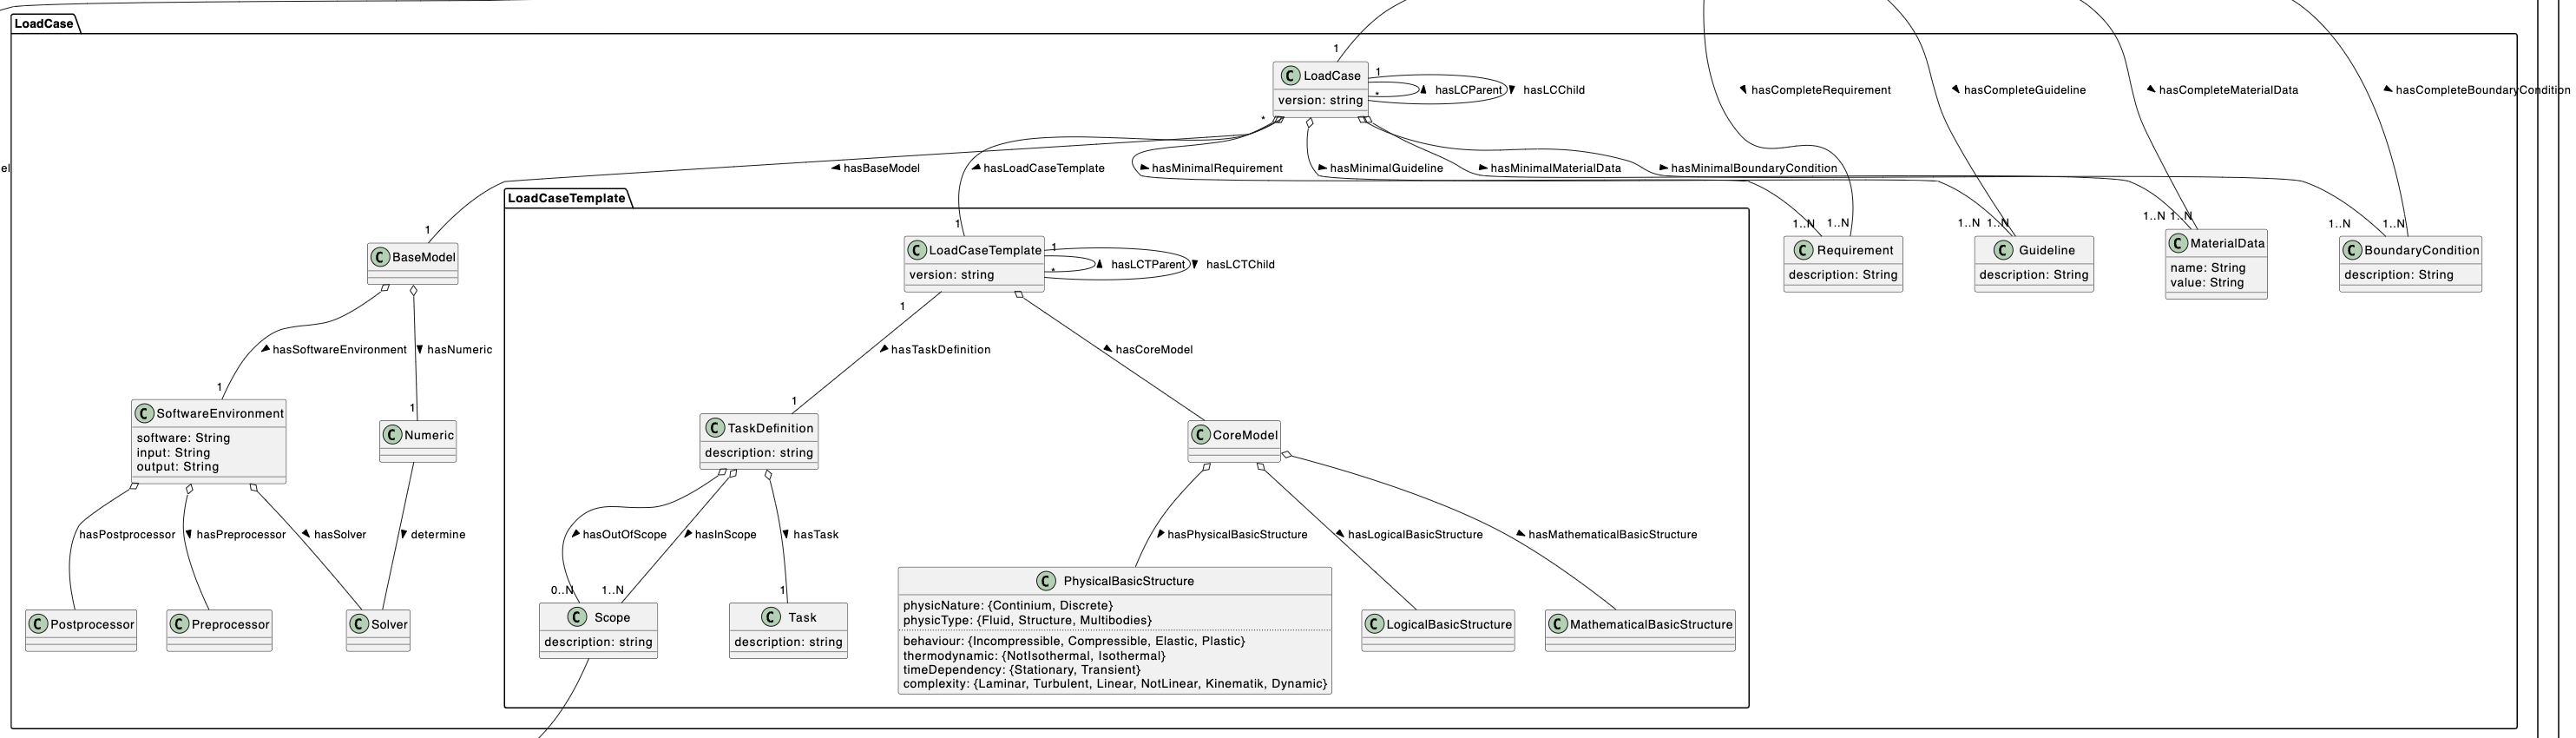
\includegraphics[width=\textwidth]{images/UML-Sim.png}
    \caption{\label{fig:uml-sim}  UML representation of the simulation’s metadata}
\end{figure}


\subsection{Simulation Modeling using Ontology}
There is no single technique for modeling a domain; there are always valid options. The ideal method is almost always determined by the application and extensions you intend to implement. Ontology development is an iterative process. Ontology concepts need to be linked to objects (physical or logical) and relationships in your field of interest. These objects are most likely to be nouns (things) or verbs (relations) in the sentences describing your domain. As presented in Section\ref{para:sms_analysis}, the researchers behind the "Protégé" software have put together a set of best practices, which will be followed in this work []. The steps to follow are:

\begin{itemize}
    \item Step1: Scope Definition
    \item Step2: Reuse Existing Vocabulary
    \item Step3: Identification of Important Terms
    \item Step4: Class Hierarchy and Taxonomy
    \item Step5: Define Attributes and Properties of Classes — Slots
    \item Step6: Define the Facets of the Slots
    \item Step7: Creation of Instances
\end{itemize}

    \subsubsection{Step1: Scope Definition}
    The development of an ontology begins with the definition of its domain and field of application. To do this, few questions need to be answered []:
    
    \begin{itemize}
        \item What domain will the ontology cover? 
        \item For what purpose will we utilize the ontology? 
        \item To what kinds of queries should the knowledge in the ontology offer answers? 
        \item Who will utilize and maintain the ontology?
    \end{itemize}
    
    The answers to these questions have already been partially addressed in our previous analysis. In this thesis, an ontology will be created to model simulations and their metadata used during configuration. The aim of the ontology is to provide a formalism for the elements involved in the configuration process, and to model the relationships and interdependencies between these elements. Different simulation templates will be stored in the ontology, and information about them can be accessed using SPARQL queries (explained in Section\ref{para:sparql}). This will enable a suitable algorithm to provide assistance to future users. The ontology will be used primarily by simulation engineers. It will be maintained by an expert in semantic technology and expert simulation engineers, who will enrich it with their knowledge.

    
    \subsubsection{Step2: Reuse Existing Vocabulary}
    Setting up an ontology from scratch can be a rather tedious and complex process, requiring a certain level of knowledge in the target domain. That's why it's worth investigating whether there's a similar ontology to the one you want to build, which can be extended and refined to meet your requirements 100\%. Numerous ontologies are available in electronic form on the Internet. Platforms such as \textbf{DBPedia}, \textbf{WikiData} or \textbf{Linked Open Vocabularies (LOV)} allow you to access free ontologies, download them and integrate them into other ontologies.\\
    
    During the study in Chapter\ref{sec:relwork}, a number of simulation ontologies were identified. These include: OSMO [], I2Sim [], OntologySim[] and VIO[]. Unfortunately, given that the elements we want to model (see Figure\ref{fig:cea-proc}) come from conventions defined as part of the EP4.0 project [], it was impossible to find a free ontology that could cover our needs. The ontology will therefore have to be built from scratch, using the structure described in Figure\ref{fig:uml-sim}.


    \subsubsection{Step3: Identification of Important Terms}
    All the important terms can be extracted from the diagram in Figure[]. The most important are:
    \begin{itemize}
        \item LoadCase Template
        \item LoadCase
        \item Basic Model
        \item Core Model
        \item Numeric 
        \item Solver
        \item Physical Basic Structure
        \item Mathematical Basic Structure
        \item Logical Basic Structure
        \item Task
    \end{itemize}

    
    \subsubsection{Step4: Class Hierarchy and Taxonomy}
    There are three main techniques for building a class hierarchy.
    \begin{itemize}
        \item \textbf{A top-down development}: this method begins with the formulation of the most general notions of the domain, followed by the specialization of these concepts.
        \item \textbf{A bottom-up development}: this begins with the definition of the most detailed classes in the hierarchy, then groups these classes into more generic notions.
        \item \textbf{A combination development}: this method combines the two previous approaches. The most important ideas are first identified. They are then generalized and specified as appropriate.
    \end{itemize}
    
    For the purposes of this thesis, the third (hybrid) approach is the most appropriate. Since the majority of key elements have already been defined (top-down), it remains to group those of the same type into more generic notions (bottom-up). The various intermediates elements / classes are presented in the following diagrams:
    
    \begin{figure}
        \centering
            \begin{tikzpicture} 
            \centering
            \umlsimpleclass{Package} 
            \umlsimpleclass[x=-2, y=-2, anchor=north]{LoadCaseTemplate} 
            \umlsimpleclass[x=2, y=-2, anchor=north]{LoadCase} 
            \umlVHVinherit[arm2=-1.2cm]{LoadCaseTemplate}{Package} 
            \umlVHVinherit[arm2=-1.2cm]{LoadCase}{Package} 
            \end{tikzpicture} 
        \caption{\label{fig:distro-art} Classification of “Package”}
    \end{figure}
    
    \begin{figure}
        \centering
            \begin{tikzpicture} 
            \centering
            \umlsimpleclass{Model} 
            \umlsimpleclass[x=-2, y=-2, anchor=north]{BasicModel} 
            \umlsimpleclass[x=2, y=-2, anchor=north]{CoreModel} 
            \umlVHVinherit[arm2=-1.2cm]{BasicModel}{Model} 
            \umlVHVinherit[arm2=-1.2cm]{CoreModel}{Model} 
            \end{tikzpicture} 
        \caption{\label{fig:distro-art} Classification of “Model”}
    \end{figure}
    
    \begin{figure}
        \centering
            \begin{tikzpicture} 
            \centering
            \umlsimpleclass{BasicStructure} 
            \umlsimpleclass[x=-2, y=-2, anchor=north]{PhysicalBasicStructure} 
            \umlsimpleclass[x=4, y=-2, anchor=north]{MathematicalBasicStructure}  
            \umlsimpleclass[x=10, y=-2, anchor=north]{LogicalBasicStructure} 
            \umlVHVinherit[arm2=-1.2cm]{PhysicalBasicStructure}{BasicStructure} 
            \umlVHVinherit[arm2=-1.2cm]{MathematicalBasicStructure}{BasicStructure} 
            \umlVHVinherit[arm2=-1.2cm]{LogicalBasicStructure}{BasicStructure} 
            \end{tikzpicture} 
        \caption{\label{fig:distro-art} Classification of “BasicStructure”}
    \end{figure}
    

    
    \subsubsection{Step5: Define Attributes and Properties of Classes — Slots}
    In order to achieve a complete, connected knowledge model, the properties of the various classes and the relationships between these classes still need to be explicitly defined. Here again, our UML diagram in Figure\ref{fig:uml-sim} comes into play. It contains the definition of each class and their properties.
    
    
    \subsubsection{Step6: Define the Facets of the Slots}
    Slots can have many facets that describe the type of value, the permitted values, the number of values (cardinality) and other characteristics of the values the slot can accept. A facet can be a string, a number, a Boolean literal or an instance of a class. The "range" represents the classes authorized for the value of a property. And the "domain" represents the classes that a property can describe. The diagram in Figure\ref{fig:uml-sim} also shows the relationships between the various classes, as well as their cardinalities.
    
    
    \subsubsection{Step7: Creation of Instances}
    For our purposes, instances will be created using a migration system when our server is first launched (see Chapter\ref{sec:implementation}).
    

\subsection{Reasoning Mechanisms}
    \subsubsection{Case-Based reasoning}
        \paragraph{Retrieve}
        
        \paragraph{Reuse}
        
        \paragraph{Revise}
        
        \paragraph{Retain}
    
    \subsubsection{Rule-Based reasoning}
        \paragraph{First Order Logic (FOL)}

